% =====================================================================
% Short paper - Churn em e-commerce
% Aluno: João Gabriel Tavares Silva - Matrícula 221021071 - UnB
% Classe abnTeX2 (ABNT NBR 6022:2018 - artigo científico)
% Compilar com pdfLaTeX + BibTeX (padrão do Overleaf)
% =====================================================================
\documentclass[
  article,            % artigo acadêmico
  12pt,
  oneside,
  a4paper,
  section=TITLE,      % seções primárias em maiúsculas
  english,            % idioma adicional (abstract)
  brazil              % idioma principal
]{abntex2}

\usepackage[T1]{fontenc}
\usepackage[utf8]{inputenc}
\usepackage{times}              % fonte Times (ABNT)
\usepackage{indentfirst}
\usepackage{graphicx}
\usepackage{microtype}
\usepackage{booktabs}
\usepackage{tabularx}
\usepackage{float}
\usepackage{amsmath}
\usepackage[alf]{abntex2cite}   % citações autor-data (ABNT NBR 10520)

\graphicspath{{figuras/}}

% ---------- Dados do documento ----------
\titulo{Churn em e-commerce: auditoria de dados, correlações entre fatores e modelos de cancelamento}
\tituloestrangeiro{E-commerce churn: data audit, correlations between factors and cancellation models}
\autor{João Gabriel Tavares Silva}
\local{Brasília}
\data{2026}

\makeatletter
\hypersetup{
  pdftitle={\@title},
  pdfauthor={\@author},
  pdfsubject={Short paper - churn em e-commerce},
  colorlinks=true, linkcolor=black, citecolor=black, urlcolor=blue
}
\makeatother

% ---------- Layout ABNT ----------
\setlrmarginsandblock{3cm}{2cm}{*}
\setulmarginsandblock{3cm}{2cm}{*}
\checkandfixthelayout
\setlength{\parindent}{1.25cm}
\setlength{\parskip}{0.2cm}
\OnehalfSpacing

% Títulos em Times negrito (seções primárias em maiúsculas pela opção section=TITLE)
\renewcommand{\ABNTEXchapterfont}{\rmfamily\bfseries}
\renewcommand{\ABNTEXchapterfontsize}{\normalsize}
\renewcommand{\ABNTEXsectionfont}{\rmfamily\bfseries}
\renewcommand{\ABNTEXsectionfontsize}{\normalsize}
\renewcommand{\ABNTEXsubsectionfont}{\rmfamily\bfseries}
\renewcommand{\ABNTEXsubsectionfontsize}{\normalsize}

% Tabelas: texto menor e espaçamento simples
\newcommand{\tabelaabnt}{\footnotesize\SingleSpacing}

\begin{document}
\selectlanguage{brazil}
\frenchspacing
\renewcommand{\resumoname}{RESUMO}
\renewcommand{\bibname}{REFERÊNCIAS}
\renewcommand{\refname}{REFERÊNCIAS}

% ---------- Cabeçalho com logo da UnB ----------
\begin{center}
  
\includegraphics[width=3cm]{logo-unb}\\[0.6cm]
  {\large\bfseries Churn em e-commerce: auditoria de dados, correlações entre fatores e modelos de cancelamento\par}
  \vspace{0.6cm}
  {\normalsize João Gabriel Tavares Silva\footnote{Aluno da Universidade de Brasília (UnB). Matrícula: 221021071.}\par}
  {\small Universidade de Brasília (UnB)\par}
\end{center}
\vspace{0.4cm}

% ---------- Resumo ----------
\begin{resumoumacoluna}
  \SingleSpacing
  Este trabalho analisa uma base pública de 50.000 clientes de comércio eletrônico, com 25 variáveis de perfil, engajamento, compras e atrito, para identificar fatores associados ao cancelamento (\textit{churn}), que atinge 28,9\% dos clientes. A auditoria mostrou que a base é simulada: dados faltantes em proporções redondas exatas, geografia e cadastro distribuídos de forma perfeita e 451 clientes com valores impossíveis inseridos. Os resultados valem, portanto, como estudo de método. Valores extremos distorcem a correlação de Pearson (ticket médio $\times$ valor do cliente: 0,15 em Pearson, 0,56 em Spearman). Um único fator de engajamento explica 36,5\% da variância das 20 variáveis numéricas, e, controlado esse fator, as oito medidas de engajamento perdem quase toda a correlação com o churn. Os sinais mais fortes são de atrito: o churn vai de 12\% a 47\% entre o quintil mais baixo e o mais alto de ligações ao atendimento. Um modelo de \textit{gradient boosting} (AUC = 0,93) supera a regressão logística (AUC = 0,79) porque capta relações não lineares, como o churn em forma de U ao longo do valor do cliente.

  \vspace{\onelineskip}
  \noindent
  \textbf{Palavras-chave}: churn; comércio eletrônico; qualidade de dados; correlação; gradient boosting.
\end{resumoumacoluna}

\renewcommand{\resumoname}{ABSTRACT}
\begin{resumoumacoluna}
  \SingleSpacing
  \begin{otherlanguage*}{english}
    This paper analyzes a public dataset of 50,000 e-commerce customers, with 25 profile, engagement, purchase and friction variables, to identify factors associated with churn, which affects 28.9\% of customers. The audit showed that the dataset is simulated: missing values in exact round proportions, perfectly balanced geography and sign-up dates, and 451 customers with injected impossible values. The results therefore stand as a methodological study. Extreme values distort Pearson correlation (average order value $\times$ customer value: 0.15 in Pearson, 0.56 in Spearman). A single engagement factor explains 36.5\% of the variance of the 20 numeric variables, and, once it is controlled for, the eight engagement measures lose almost all their correlation with churn. The strongest signals relate to friction: churn rises from 12\% to 47\% between the lowest and highest quintile of customer service calls. A gradient boosting model (AUC = 0.93) outperforms logistic regression (AUC = 0.79) because it captures non-linear relationships, such as the U-shaped churn along customer lifetime value.

    \vspace{\onelineskip}
    \noindent
    \textbf{Keywords}: churn; e-commerce; data quality; correlation; gradient boosting.
  \end{otherlanguage*}
\end{resumoumacoluna}

\textual

% =====================================================================
\section{Introdução}

Reter um cliente costuma custar menos do que conquistar outro, e por isso prever o cancelamento (\textit{churn}) é um dos usos mais comuns de dados em comércio eletrônico. Bases públicas de churn circulam amplamente em plataformas como o Kaggle e são usadas em cursos e trabalhos acadêmicos, muitas vezes sem verificação da origem ou da qualidade dos dados.

O trabalho responde a três perguntas. Primeiro, a base é confiável e o que precisa ser corrigido antes da análise? Segundo, como os fatores de perfil, engajamento, compras e atrito se relacionam entre si? Terceiro, quais fatores estão associados ao churn, e essa associação é linear?

A contribuição é metodológica. O trabalho mostra como identificar uma base simulada, como valores extremos e variáveis redundantes enganam a análise de correlação e por que modelos lineares podem esconder o fator mais importante. O código completo e interativo está em um notebook público \cite{silva2026churn}.

% =====================================================================
\section{Dados e método}

\subsection{Base de dados}

A base reúne 50.000 clientes de uma loja on-line em 8 países e 40 cidades \cite{srisyra2026}. As 25 variáveis foram agrupadas em quatro blocos: perfil (idade, gênero, país, tempo de cadastro), engajamento (logins, duração da sessão, páginas, app, e-mails, redes sociais, lista de desejos, avaliações), compras (total, ticket médio, recência, descontos, devoluções, meios de pagamento, valor do cliente ou LTV, saldo de crédito) e atrito (abandono de carrinho, ligações ao atendimento). A variável de interesse indica se o cliente cancelou; a taxa geral é de 28,9\%. Não há datas, apenas o trimestre de cadastro, o que faz da base um corte transversal.

\subsection{Auditoria}

A conferência da base encontrou sinais consistentes de geração sintética (Tabela~\ref{tab:simulada}).

\begin{table}[htbp]
  \centering
  \caption{Evidências de que a base é simulada}
  \label{tab:simulada}
  \tabelaabnt
  \begin{tabularx}{\textwidth}{>{\raggedright\arraybackslash}p{5cm} >{\raggedright\arraybackslash}X}
    \toprule
    \textbf{Evidência} & \textbf{O que se observa} \\
    \midrule
    Faltantes em proporções redondas & 5,0\%, 6,0\%, 7,0\%, 8,0\%, 10,0\%, 11,0\% e 12,0\% em colunas diferentes \\
    Geografia artificial & Exatamente 5 cidades por país, sempre as maiores \\
    Cadastro uniforme & Entre 24,9\% e 25,1\% dos clientes em cada trimestre \\
    Erros inseridos & Idades de 5, 10, 150 e 200 anos; compras negativas; taxas acima de 100\% (451 clientes no total) \\
    Contagem com decimais & 22,5\% dos clientes com total de compras fracionário \\
    Correlações do tipo tudo ou nada & Dos 190 pares, 111 com correlação abaixo de 0,1 em módulo, 78 acima de 0,3 e só 1 entre os dois \\
    \bottomrule
  \end{tabularx}
  \fonte{Elaboração própria a partir de \citeonline{srisyra2026}.}
\end{table}

A falta de dado não é aleatória em duas variáveis. Clientes sem duração de sessão registrada têm churn de 41,1\%, contra 28,0\% dos demais; sem taxa de abertura de e-mails, 40,7\% contra 28,3\% (qui-quadrado com correção de Benjamini e Hochberg, $p < 0{,}001$). Excluir essas linhas enviesaria a análise \cite{little2019}.

\subsection{Limpeza}

Valores impossíveis (idade fora de 16 a 100 anos, compras negativas, taxas acima de 100\%) foram convertidos em faltantes. Extremos plausíveis, como tickets acima de US\$~1.000, foram mantidos, e por isso as análises usam medidas robustas a eles. Nos modelos, faltantes foram imputados pela mediana com uma variável indicadora de falta.

\subsection{Medidas e modelos}

As correlações entre os 190 pares de variáveis numéricas foram medidas por Pearson e por \citeonline{spearman1904}, que usa a ordem dos valores e resiste a extremos, com correção de \citeonline{benjamini1995} para múltiplas comparações. A estrutura comum foi estimada por componentes principais, e a correlação parcial com o churn foi calculada controlando o primeiro componente. As variáveis categóricas foram avaliadas pelo V de \citeonline{cramer1946}.

Para o churn, compararam-se uma regressão logística com variáveis padronizadas e um modelo de \textit{gradient boosting} \cite{friedman2001}, ambos por validação cruzada estratificada em cinco partes e medidos pela área sob a curva ROC (AUC). A importância das variáveis foi medida por permutação em uma amostra de teste de 25\%.

% =====================================================================
\section{Resultados}

\subsection{Correlações entre pares}

Valores extremos alteram a correlação de Pearson nos dois sentidos. Entre ticket médio e valor do cliente (LTV), Pearson indica 0,15 e Spearman 0,56: 25 tickets acima de US\$~1.000 achatam a relação linear. Entre total de compras e taxa de devolução ocorre o inverso: Pearson indica 0,28, criado por poucos extremos, e Spearman 0,01. Por isso as análises seguintes usam Spearman na base limpa.

As variáveis formam um bloco fortemente ligado (Figura~\ref{fig:heatmap}). Os pares mais fortes são total de compras $\times$ LTV ($\rho = 0{,}75$), duração da sessão $\times$ páginas por sessão (0,74) e duração da sessão $\times$ uso do app (0,74). O abandono de carrinho é o espelho negativo desse bloco: $\rho = -0{,}69$ com a duração da sessão. O primeiro componente principal, um fator de engajamento, explica 36,5\% da variância das 20 variáveis, contra cerca de 5\% se elas fossem independentes.

\begin{figure}[htbp]
  \centering
  \caption{Correlação de Spearman entre as 20 variáveis numéricas, ordenadas por agrupamento hierárquico}
  \label{fig:heatmap}
  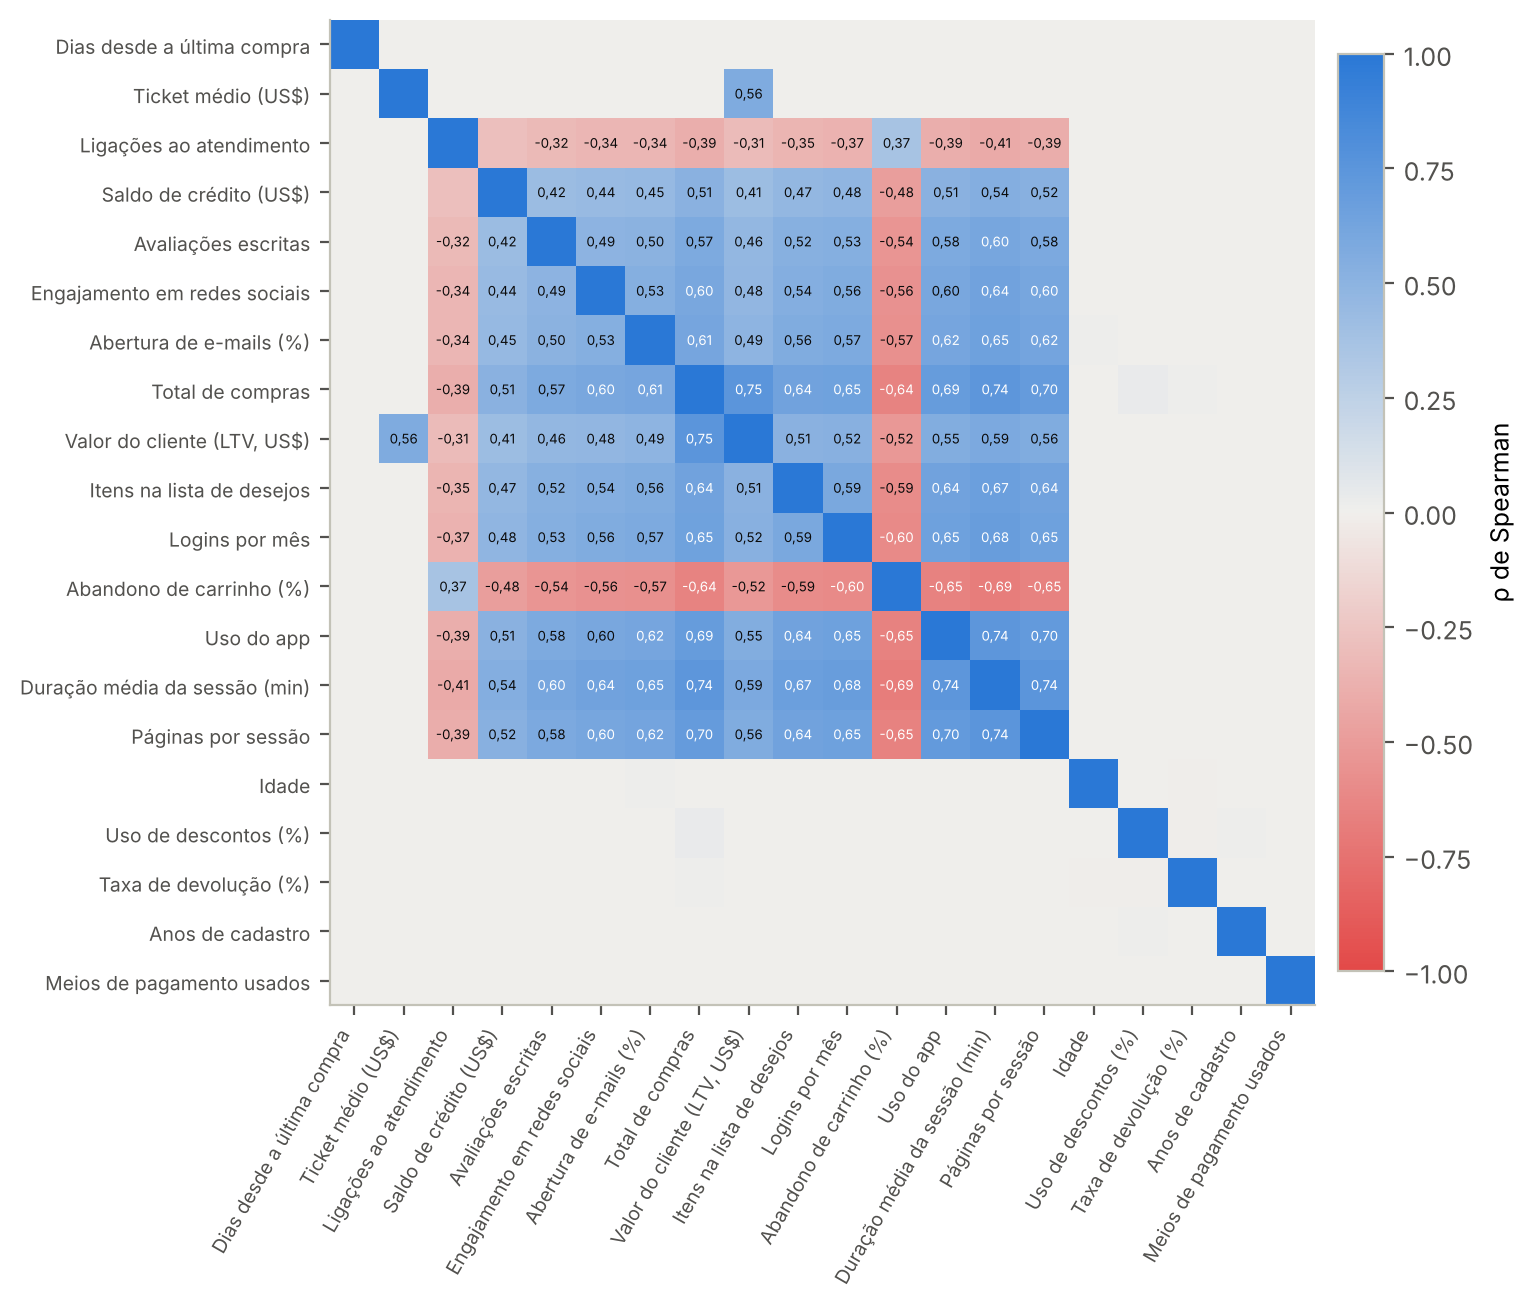
\includegraphics[width=0.92\textwidth]{f1_heatmap}
  \fonte{Elaboração própria a partir de \citeonline{srisyra2026}. Valores exibidos apenas quando o módulo de $\rho$ é de pelo menos 0,3.}
\end{figure}

O perfil demográfico praticamente não se relaciona com o churn. Entre países, a taxa vai de 27,3\% a 29,9\%; entre gêneros, de 28,7\% a 31,3\%; e o V de Cramér fica abaixo de 0,02 em país, gênero e trimestre de cadastro.

\subsection{Fatores associados ao churn}

A correlação bruta com o churn é negativa para todas as medidas de engajamento, entre $-0{,}20$ e $-0{,}24$. Controlado o fator de engajamento, porém, essas correlações caem para perto de zero (Figura~\ref{fig:parcial}): as oito variáveis medem a mesma coisa. Os fatores que mantêm associação própria são as ligações ao atendimento, o ticket médio, a recência da última compra e a idade (Tabela~\ref{tab:quintis}).

\begin{figure}[htbp]
  \centering
  \caption{Correlação de Spearman com o churn: bruta e parcial (controlado o fator de engajamento)}
  \label{fig:parcial}
  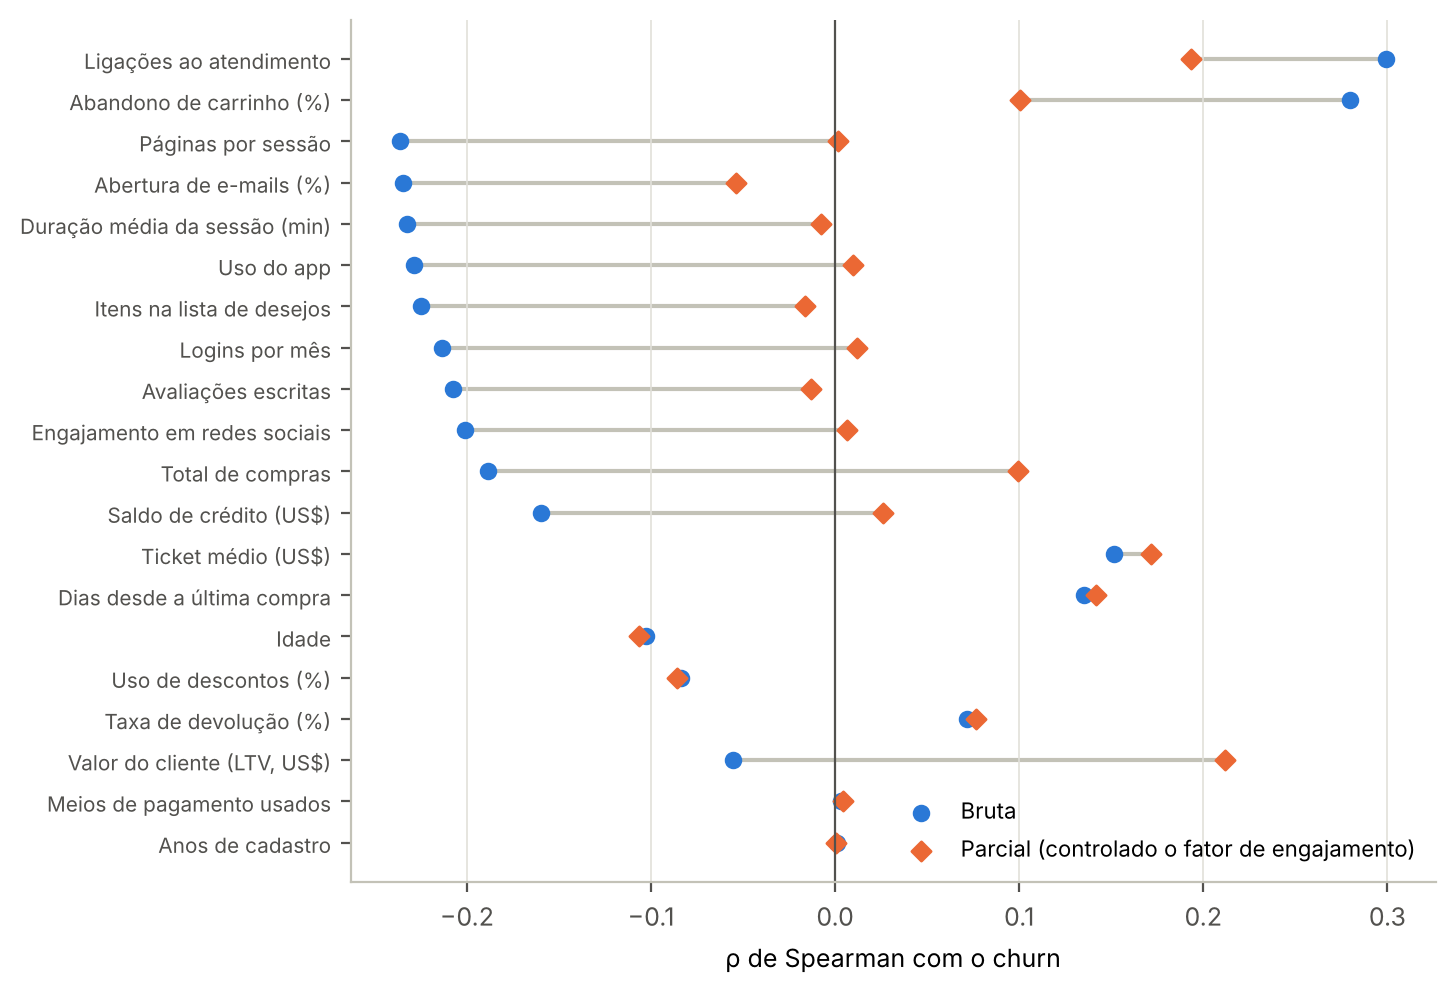
\includegraphics[width=0.85\textwidth]{f2_parcial}
  \fonte{Elaboração própria a partir de \citeonline{srisyra2026}.}
\end{figure}

\begin{table}[htbp]
  \centering
  \caption{Churn por quintil e correlação com o churn, variáveis selecionadas}
  \label{tab:quintis}
  \tabelaabnt
  \begin{tabular}{lcccc}
    \toprule
    \textbf{Variável} & \textbf{Churn no 1\textsuperscript{o} quintil} & \textbf{Churn no 5\textsuperscript{o} quintil} & \textbf{$\rho$ bruta} & \textbf{$\rho$ parcial} \\
    \midrule
    Ligações ao atendimento & 12\% & 47\% & +0,30 & +0,19 \\
    Abandono de carrinho & 19\% & 57\% & +0,28 & +0,10 \\
    Duração média da sessão & 49\% & 19\% & $-$0,23 & $-$0,01 \\
    Abertura de e-mails & 50\% & 18\% & $-$0,23 & $-$0,05 \\
    Dias desde a última compra & 22\% & 40\% & +0,14 & +0,14 \\
    Valor do cliente (LTV) & 45\% & 38\% & $-$0,06 & +0,21 \\
    Anos de cadastro & 28\% & 29\% & 0,00 & 0,00 \\
    \bottomrule
  \end{tabular}
  \fonte{Elaboração própria. Quintil 1 = 20\% dos clientes com menor valor da variável. Taxa média de churn: 28,9\%.}
\end{table}

O LTV merece destaque. Sua correlação com o churn é quase nula ($-0{,}06$), mas a relação tem forma de U: 45\% de churn no quintil mais baixo, 17\% no do meio e 38\% no mais alto. Uma correlação, por resumir a relação numa reta, não enxerga esse padrão. Na regressão logística, o coeficiente do LTV ainda muda de sinal (+0,81) quando o total de compras entra no modelo, um efeito de supressão: o LTV passa a medir o valor gasto por compra.

\subsection{Modelos}

O \textit{gradient boosting} teve AUC de 0,927 (desvio-padrão de 0,005 entre as cinco partes da validação cruzada), contra 0,790 (0,004) da regressão logística. A diferença de 0,14 indica que boa parte da relação com o churn é não linear. Na importância por permutação, o LTV e as ligações ao atendimento dominam: embaralhar cada um reduz o AUC em 0,16 e 0,14, respectivamente, contra 0,06 da idade e 0,05 do uso de descontos (Figura~\ref{fig:importancia}).

\begin{figure}[htbp]
  \centering
  \caption{Importância das variáveis no modelo de \textit{gradient boosting} (queda no AUC ao embaralhar cada variável)}
  \label{fig:importancia}
  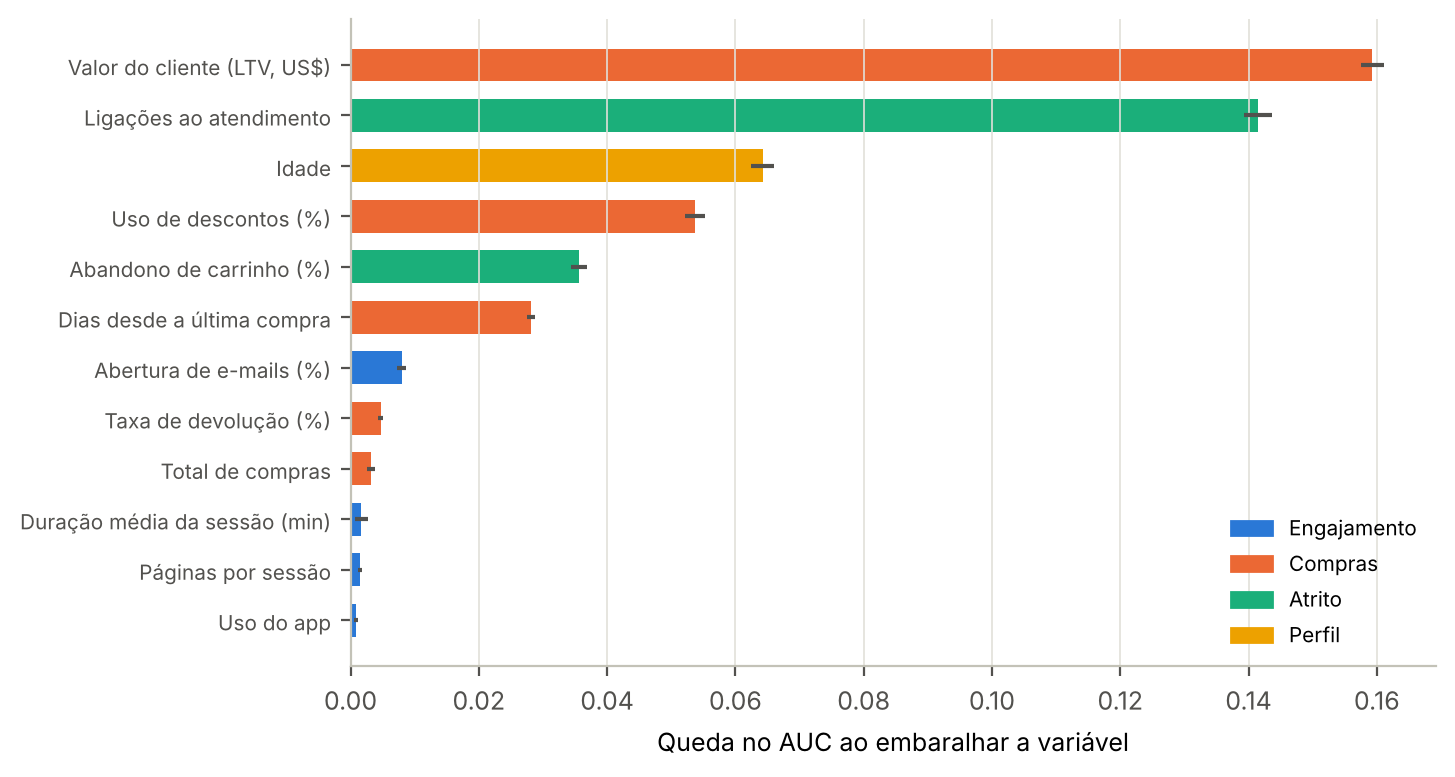
\includegraphics[width=0.85\textwidth]{f3_importancia}
  \fonte{Elaboração própria a partir de \citeonline{srisyra2026}. AUC no conjunto de teste = 0,931. As 12 variáveis mais importantes; barras de erro = desvio-padrão em 5 repetições.}
\end{figure}

A dependência parcial mostra por que o modelo de árvores vence: os efeitos são degraus, não retas (Figura~\ref{fig:degraus}). O churn previsto salta de 19\% para 43\% entre 5 e 6 ligações ao atendimento e de 21\% para 56\% quando o LTV passa de cerca de US\$~1.800; cai de 47\% para 26\% quando a idade passa de 24 anos e de 35\% para 26\% quando o uso de descontos passa de 30\%. Degraus tão nítidos, em valores redondos, são mais um indício de que o gerador da base definiu o churn por regras de corte. Condicionado às demais variáveis, o LTV tem um único degrau; o U observado na Tabela~\ref{tab:quintis} vem de clientes de LTV baixo que também engajam menos.

\begin{figure}[htbp]
  \centering
  \caption{Dependência parcial: churn previsto ao longo das quatro variáveis mais importantes}
  \label{fig:degraus}
  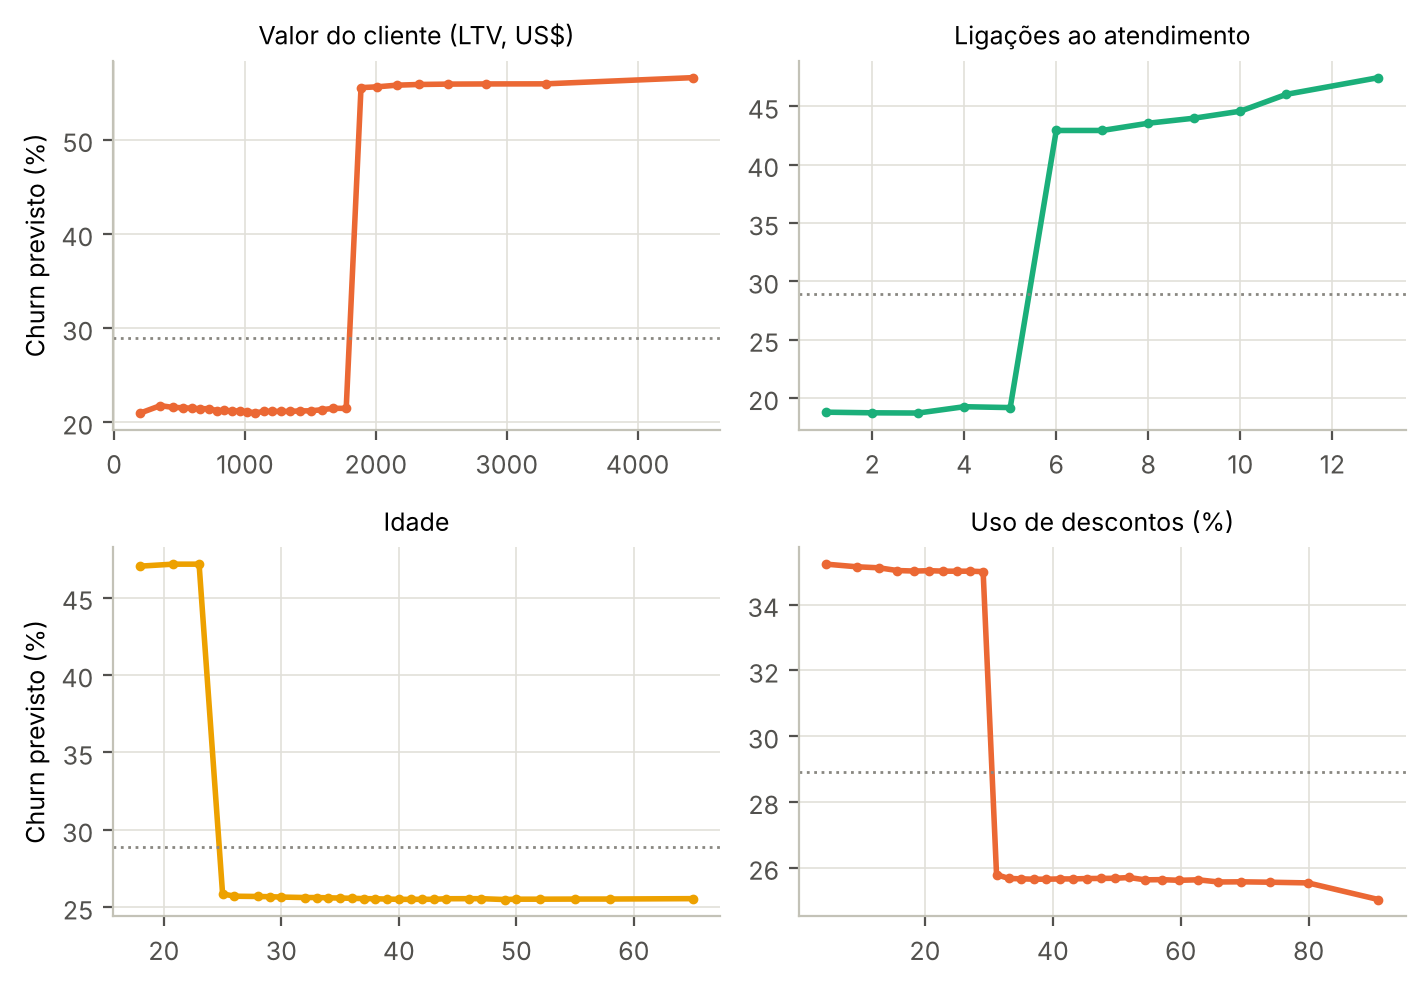
\includegraphics[width=0.92\textwidth]{f4_degraus}
  \fonte{Elaboração própria a partir de \citeonline{srisyra2026}. Linha pontilhada = taxa média de churn (28,9\%).}
\end{figure}

% =====================================================================
\section{Discussão e limitações}

O primeiro resultado é sobre a própria base. Uma auditoria simples, com contagem de faltantes, faixas de valores e distribuição das categorias, bastou para mostrar que os dados são simulados. Bases desse tipo são úteis para ensino, mas conclusões sobre o comportamento de consumidores reais exigiriam dados coletados. A auditoria também revelou que a falta de dado carrega informação: descartar as linhas incompletas teria retirado justamente clientes com mais churn.

O segundo resultado é sobre a leitura de correlações. Oito variáveis de engajamento parecem fatores distintos de retenção quando vistas uma a uma, mas são versões de um mesmo comportamento. Para a gestão, isso significa que acompanhar oito indicadores de engajamento acrescenta pouco a acompanhar um índice que os resuma. Já os sinais de atrito, como ligações ao atendimento e abandono de carrinho, têm associação própria com o churn e apontam para pontos de intervenção no processo de atendimento e de compra.

O terceiro resultado é sobre modelos. A regressão logística é interpretável, mas supõe efeitos lineares e perdeu 0,14 de AUC para o modelo de árvores. O caso do LTV mostra o custo dessa suposição: a variável mais importante do modelo não linear parecia irrelevante na correlação e tinha coeficiente de sinal contraintuitivo na regressão.

Há três limitações principais. A base é simulada, e as relações encontradas refletem as regras do gerador dos dados. Os dados são de corte transversal, sem datas, o que impede saber se a queda de engajamento antecede o cancelamento. E associação não implica causalidade: ligações ao atendimento podem ser sintoma, e não causa, da insatisfação.

% =====================================================================
\section{Conclusão}

A base analisada é simulada, e reconhecer isso foi o primeiro resultado do trabalho. Nela, o churn de 28,9\% não depende do perfil demográfico, mas de um fator geral de engajamento, de sinais de atrito (ligações ao atendimento e abandono de carrinho) e, de forma não linear, do valor do cliente. Três cuidados de método mudaram as conclusões: usar correlações robustas a extremos, controlar variáveis redundantes e testar modelos não lineares. Sem eles, o fator mais importante do churn, o LTV, teria parecido irrelevante.

% ---------- Referências ----------
\postextual
\bibliography{referencias}

\end{document}
